\documentclass[11pt, a4paper, norsk]{NTNUoving}
\usepackage[utf8]{inputenc}
\usepackage[T1]{fontenc}
\usepackage{tikz}

\ovingnr{4}    % Nummer på innlevering
\semester{Høsten 2019} % husk å bytte denne
\fag{TMA 4115} %4105 er matte 2, 4115 er matte 3
\institutt{Institutt for matematiske fag}

% bruker noen ganger denne fordi "punkt" noen ganger ikke vil autocomplete
\newenvironment{pkt}{\begin{punkt}}{\end{punkt}}

% eksempel på bruk kommer litt under
\newenvironment{matrise}[1][c]{
        \left[
            \begin{array}{#1}
    }
    {    
    \end{array}
    \right]           
}

% indreprodukt-klammer rundt det inni denne
\newenvironment{indreprod}{
    \langle
}{
\rangle}

% bruk \R inni math mode for å få mengden av reelle tall
\newcommand{\R}{\mathbb{R}}
% bruk \P for kaligrafisk P (polynomer)
\renewcommand{\P}{\mathcal{P}}

\begin{document}
%#################################################
%Dette er for enkel copy-pasting
% alt mellom \ifx og \fi tegnes ikke
\ifx
%-------------------------
\begin{oppgave}
    \begin{punkt}
        \begin{align*}
        
        
        \end{align*}
    \end{punkt}
\end{oppgave}
%-------------------------
\begin{tikzpicture}
    \draw[step=1cm,gray,very thin] (-2.9,-2.9) grid (2.9,2.9);
    \draw (-3,0) -- (3,0); % x-akse
    \draw (0,-3) -- (0,3); % y-akse
    \draw[->] (-3,0) -- (3,0); % vektoren fra (-3, 0) til (3, 0)
    \draw[->] (0,-3) -- (0,3);
    \draw (0, 3.1) node {Im}; % "Im" kan byttes med "y" om man ønsker kartesiske heller enn komplekse koordinater
    \draw (3.1, 0) node {Re};
\end{tikzpicture}

\begin{align*}
    \begin{matrise}[ccc|c] % med streken blir det en totalmatrise for et ligningssystem. Bare å prøve
        1 & 2 & 3 & 4 \\
        2 & 3 & 4 & 5 \\
        3 & 4 & 5 & 6
    \end{matrise}
\end{align*}
\fi

%Her begynner dokumentet
%#####################################
\begin{oppgave}
    \begin{punkt}
        Indreproduktet for vektorene er skalarprodukt. Vektorer er ortogonale dersom indreproduktet er lik 0.
        \begin{align*}
            \begin{matrise}[c]
                2\\-5\\1
            \end{matrise}
            \cdot
            \begin{matrise}[c]
                1\\2\\0
            \end{matrise}
        = 2\cdot 1 - 5 \cdot 2 + 1\cdot 0 \neq 0
        \end{align*}
    \end{punkt}
    \begin{punkt}
        Her ser vi at skalarproduktet blir 0 for alle vektorene. De er dermed ortogonale.
    \end{punkt}
    \begin{punkt}
        Med komplekse vektorer må en av dem komplekskonjugeres. Det gir at $\begin{matrise}[c]
            1\\i\\i
        \end{matrise}$ er ortogonal med de to andre, men de to andre er ikke ortogonale med hverandre.
    \end{punkt}
\end{oppgave}
\begin{oppgave}
    \begin{punkt}
        \begin{align*}
            u_1 &=v_1 = \begin{matrise}[c]2\\-5\\1\end{matrise}\\
            u_2 &=v_2-\frac{u_1\cdot v_2}{u_1 \cdot u_1}u_1
             \\ &=\begin{matrise}[c]1\\2\\0\end{matrise}-\frac{\begin{matrise}[c]2\\-5\\1\end{matrise}\cdot \begin{matrise}[c]1\\2\\0\end{matrise}}{\begin{matrise}[c]2\\-5\\1\end{matrise} \cdot \begin{matrise}[c]2\\-5\\1\end{matrise}}\begin{matrise}[c]2\\-5\\1\end{matrise}
             \\&=\begin{matrise}[c]1\\2\\0\end{matrise}+\frac{8}{30}\begin{matrise}[c]2\\-5\\1\end{matrise}
             \\&=\frac{1}{30}\begin{matrise}[c]46\\20\\8\end{matrise}
        \end{align*}
    \end{punkt}
    \begin{punkt}
        Ettersom disse allerede er ortogonale vil Gram-Schmidts metode gi de samme vektorene. 
    \end{punkt}
    \begin{punkt}
        \begin{align*}
            u_1 &=\begin{matrise}[c]
            i\\0\\1
            \end{matrise}
            \\u_2 &=\begin{matrise}[c]
            1\\i\\i
            \end{matrise}
            \\u_3 &=\begin{matrise}[c]
            i\\1\\0
            \end{matrise}
            -\frac{\begin{matrise}[c]
            -i\\0\\1
            \end{matrise}\cdot \begin{matrise}[c]
            i\\1\\0
            \end{matrise}}{\begin{matrise}[c]
            -i\\0\\1
            \end{matrise}\cdot \begin{matrise}[c]
            i\\0\\1
            \end{matrise}}\begin{matrise}[c]
            i\\0\\1
            \end{matrise}
            -\frac{\begin{matrise}[c]
            1\\-i\\-i
            \end{matrise}\cdot \begin{matrise}[c]
            i\\1\\0
            \end{matrise}}{\begin{matrise}[c]
            1\\-i\\-i
            \end{matrise}\cdot \begin{matrise}[c]
            1\\i\\i
            \end{matrise}}\begin{matrise}[c]
            1\\i\\i
            \end{matrise}
            \\&=\begin{matrise}
                i\\1\\0
            \end{matrise}
            -\frac{1}{2} \begin{matrise}[c]
            i\\0\\1
            \end{matrise}
            \\&=\frac{1}{2}\begin{matrise}
            i\\2\\-1
            \end{matrise}
        \end{align*}
    \end{punkt}
\end{oppgave}
\begin{oppgave}
    \begin{pkt}
        \begin{align*}
            P_{a_1}\left(\begin{matrise}
            1\\2\\3
            \end{matrise}\right)&=\frac{a_1\cdot \begin{matrise}
            1\\2\\3
            \end{matrise}}{a_1\cdot a_1}a_1
            \\&= \frac{2\cdot 1 - 5 \cdot 2 + 1 \cdot 3}{4+25+1}\begin{matrise}
                2\\-5\\1
            \end{matrise}
            \\&=\frac{-5}{30}\begin{matrise}
                2\\-5\\1
            \end{matrise}
        \end{align*}
        \begin{align*}
            P_{a_2}\left(\begin{matrise}
            1\\2\\3
            \end{matrise}\right)&=\frac{a_2\cdot \begin{matrise}
            1\\2\\3
            \end{matrise}}{a_2\cdot a_2}a_2
            \\&= \frac{1+4}{1+4}\begin{matrise}
            1\\2\\0
            \end{matrise}
            \\&=\begin{matrise}
            1\\2\\0
            \end{matrise}
        \end{align*}
        For de to andre deloppgavene er det bare å gjøre det samme. 
    \end{pkt}
\end{oppgave}

\begin{oppgave}
    \begin{align*}
        P_\textbf{v}(\textbf{u})&=\frac{\textbf{v}\cdot \textbf{u}}{\textbf{v}\cdot \textbf{v}}\textbf{v}
        \\&= \frac{1\cdot 2 -5\cdot 2}{1+4}\begin{matrise}
        1\\2
        \end{matrise}
        \\&= -\frac{8}{5}\begin{matrise}
        1\\2
        \end{matrise}
    \end{align*}
    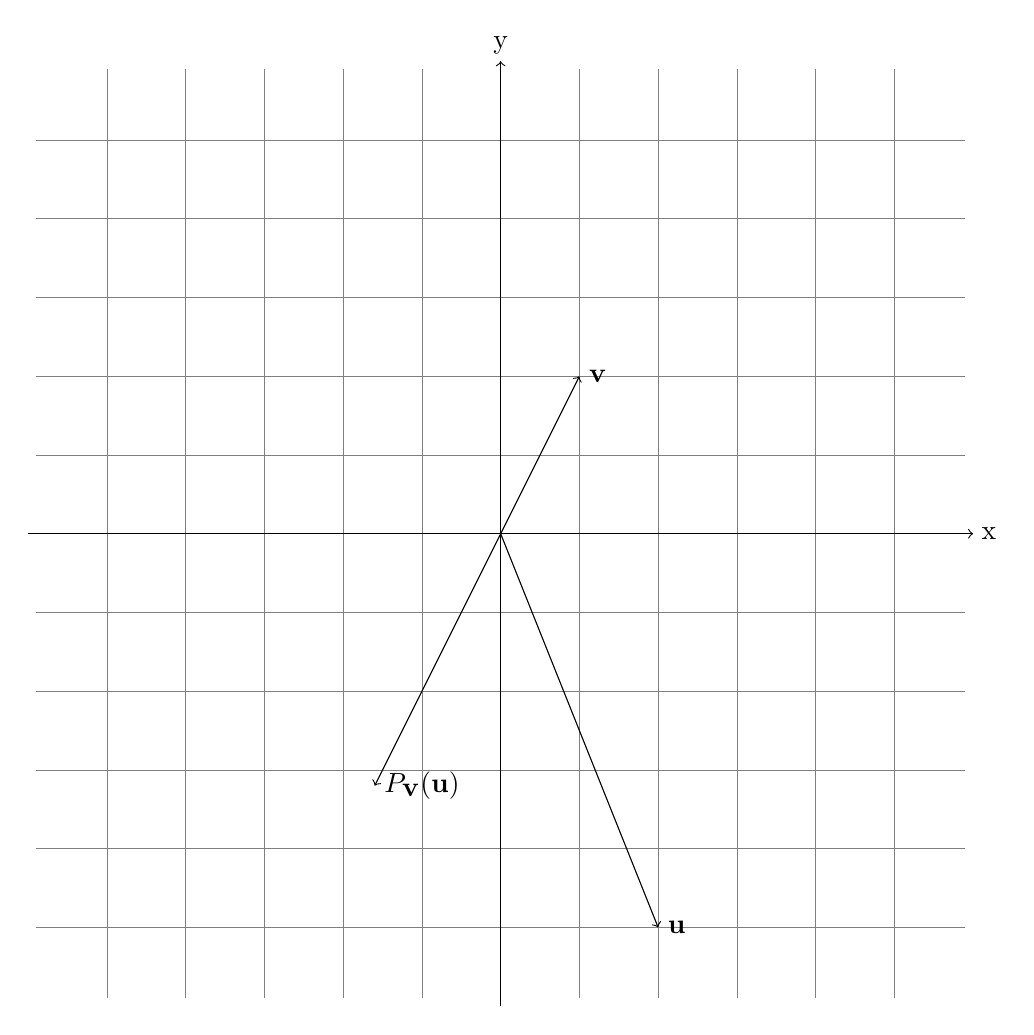
\begin{tikzpicture}
        \draw[step=1cm,gray,very thin] (-5.9,-5.9) grid (5.9,5.9);
        \draw (-6,0) -- (6,0);
        \draw (0,-6) -- (0,6);
        \draw[->] (-6,0) -- (6,0); 
        \draw[->] (0,-6) -- (0,6);
        \draw (0, 6.2) node {y};
        \draw[->] (0, 0) -- (2, -5) node[anchor=west]{\textbf{u}};
        \draw[->] (0, 0) -- (1, 2) node[anchor=west]{\textbf{v}};
        \draw[->] (0, 0) -- (-1.6, -3.2) node[anchor=west]{$P_\textbf{v}(\textbf{u})$};
        \draw (6.2, 0) node {x};
    \end{tikzpicture}
    
    Vinkelen mellom \textbf{v} og \textbf{u} er gitt ved $\arccos\frac{\textbf{u}\cdot \textbf{v}}{|\textbf{u}|\cdot |\textbf{v}|}=\arccos\frac{-8}{\sqrt{29}\cdot \sqrt{5}}=132.5^\circ$
\end{oppgave}
\begin{oppgave}
    Her innebærer de tre første deloppgave å bruke samme formel, men med litt forskjellige tall.
    \begin{align*}
        P_\textbf{u}(\textbf{v})&= \frac{\textbf{u}\cdot \textbf{v}}{\textbf{u}\cdot \textbf{u}}\textbf{u}
        \\&=\frac{2\cdot 3+2\cdot 2+1\cdot 1}{4+4+1}\begin{matrise}
        2\\2\\1
        \end{matrise}
        \\&=\frac{11}{9}\begin{matrise}
        2\\2\\1
        \end{matrise}\\
        \textbf{v}- P_\textbf{u}(\textbf{v})&=\begin{matrise}
        3\\2\\1
        \end{matrise}-\frac{11}{9}\begin{matrise}
        2\\2\\1
        \end{matrise}
        \\&=\frac{1}{9}\begin{matrise}
        5\\-4\\-2
        \end{matrise}
    \end{align*}
    \begin{align*}
        P_\textbf{u}(\textbf{v})\cdot (\textbf{v}- P_\textbf{u}(\textbf{v})) &= \frac{11}{9}\begin{matrise}
        2\\2\\1
        \end{matrise} \cdot \frac{1}{9}\begin{matrise}
        5\\-4\\-2
        \end{matrise}
        \\&=0
    \end{align*}
    Dette indreproduktet vil alltid være 0 for alle \textbf{u} og \textbf{v}. 
\end{oppgave}
\begin{oppgave}
\begin{pkt}
    \begin{align*}
        P_\textbf{v}\left( \begin{matrise}
        1\\0\\0
        \end{matrise}\right)&=\frac{1+0+0}{1+1+1}\begin{matrise}
        1\\-1\\1
        \end{matrise}
        \\&= \frac{1}{3}\begin{matrise}
        1\\-1\\1
        \end{matrise}
    \end{align*}
\end{pkt}
\begin{pkt}
    \begin{align*}
        [P_\textbf{v}]&=\begin{matrise}[c|c|c]
        P_\textbf{v}\left( \begin{matrise}
        1\\0\\0
        \end{matrise}\right) & P_\textbf{v}\left( \begin{matrise}
        0\\1\\0
        \end{matrise}\right) & P_\textbf{v}\left( \begin{matrise}
        0\\0\\1
        \end{matrise}\right)
        \end{matrise}
        \\&=\frac{1}{3}\begin{matrise}[ccc]
        1 & -1&1\\-1&1&-1\\1&-1&1
        \end{matrise}
    \end{align*}
\end{pkt}
\begin{pkt}
    Ettersom det er en projeksjon så er det uendelig mange input som gir samme output, for alle outputs. Den er altså ikke injektiv. Den er heller ikke surjektiv, ettersom funksjonen går fra $\R^3$ til $\R^3$, og output-rommet utspenner ikke $\R^3$.
\end{pkt}
\begin{pkt}
    Alle vektorer som står ortogonalt på \textbf{v} vil projiseres ned til \textbf{0}. Dimensjonen til kjernen til $P_\textbf{v}$ er da 2.
    
    $Null[P_\textbf{v}]=kerP_\textbf{v}$.
    
    Bildet blir alle vektorer parallelle med \textbf{v}. Dimenjonen er da 1.
    
    $Col[P_\textbf{v}]=imP_\textbf{v}$.
\end{pkt}
\end{oppgave}
\begin{oppgave}
    \begin{pkt}
        \begin{align*}
            u_1&=\begin{matrise}
            2\\-5\\1
            \end{matrise}
            \\u_2&=\begin{matrise}
            4\\-4\\2
            \end{matrise}
            -\frac{\begin{matrise}
            2\\-5\\1
            \end{matrise} \cdot \begin{matrise}
            4\\-4\\2
            \end{matrise}}{\begin{matrise}
            2\\-5\\1
            \end{matrise} \cdot \begin{matrise}
            2\\-5\\1
            \end{matrise}}\begin{matrise}
            2\\-5\\1
            \end{matrise}
            \\&=\begin{matrise}
            4\\-4\\2
            \end{matrise}
            -\frac{8+20+2}{4+25+1}\begin{matrise}
            2\\-5\\1
            \end{matrise}
            \\&= \begin{matrise}
            4\\-4\\2
            \end{matrise}
            -\begin{matrise}
            2\\-5\\1
            \end{matrise}
            \\&=\begin{matrise}
            2\\1\\1
            \end{matrise}
        \end{align*}
    \end{pkt}
    \begin{pkt}
    $P_W=P_{u_1}+P_{u_2}$
        \begin{align*}
            [P_W]&=\begin{matrise}[c|c|c]
            P_W\left( \begin{matrise}
            1\\0\\0
            \end{matrise}\right) & P_W\left( \begin{matrise}
            0\\1\\0
            \end{matrise}\right) & P_W\left( \begin{matrise}
            0\\0\\1
            \end{matrise}\right)
        \end{matrise}
        \end{align*}    
        \begin{align*}
            P_W\left( \begin{matrise}
            1\\0\\0
            \end{matrise}\right) &=\frac{\begin{matrise}
            2\\-5\\1
            \end{matrise} \cdot \begin{matrise}
            1\\0\\0
            \end{matrise}}{30}\begin{matrise}
            2\\-5\\1
            \end{matrise} + \frac{\begin{matrise}
            2\\1\\1
            \end{matrise} \cdot \begin{matrise}
            1\\0\\0
            \end{matrise}}{4+1+1}\begin{matrise}
            2\\1\\1
            \end{matrise}
            \\&=\frac{2}{30}\begin{matrise}
            2\\-5\\1
            \end{matrise} + \frac{2}{6}\begin{matrise}
            2\\1\\1
            \end{matrise}
            \\&=\frac{1}{30}\begin{matrise}
            4\\-10\\2
            \end{matrise} + \frac{1}{30}\begin{matrise}
            20\\10\\10
            \end{matrise}
            \\&=\frac{1}{30}\begin{matrise}
            24\\0\\12
            \end{matrise}\\
        \end{align*}
        \begin{align*}
            P_W\left( \begin{matrise}
            0\\1\\0
            \end{matrise}\right) &= \frac{-5}{30}\begin{matrise}
            2\\-5\\1
            \end{matrise} + \frac{1}{6}\begin{matrise}
            2\\1\\1
            \end{matrise}
            \\&=\frac{1}{30}\begin{matrise}
            -10\\25\\-5
            \end{matrise} + \frac{1}{30}\begin{matrise}
            10\\5\\5
            \end{matrise}
            \\&=\frac{1}{30}\begin{matrise}
            0\\30\\0
            \end{matrise}
        \end{align*}
        \begin{align*}
            P_W\left( \begin{matrise}
            0\\0\\1
            \end{matrise}\right) &= \frac{1}{30}\begin{matrise}
            2\\-5\\1
            \end{matrise} + \frac{1}{6}\begin{matrise}
            2\\1\\1
            \end{matrise}
            \\&= \frac{1}{30}\begin{matrise}
            2\\-5\\1
            \end{matrise} + \frac{1}{30}\begin{matrise}
            10\\5\\5
            \end{matrise}
            \\&=\frac{1}{30}\begin{matrise}
            12\\0\\6
            \end{matrise}
        \end{align*}
        
        Vi har da at 
        \begin{align*}
            [P_W]=\frac{1}{30}\begin{matrise}[ccc]
                24&0&12\\0&30&0\\12&0&6
            \end{matrise}
        \end{align*}
    \end{pkt}
    \begin{pkt}
        Spørsmålet her kan forenkles til hvilke vektorer som sendes til seg selv med lineærtransformasjonen $P_W$. Her er disse alle vektorer i $W$. Derfra er spørsmålet, hvilken matrise sender alle vektorer i $\R^2$ ned på $W$? Her er det bare å ta en basis for $W$. $A$ er da for eksempel $\begin{matrise}[cc]
        \textbf{u} & \textbf{v}
        \end{matrise}$.
    \end{pkt}
\end{oppgave}
\begin{oppgave}
    Her antar jeg at indreproduktet som skal brukes er $\langle p(x), q(x) \rangle=\int_0^1p(x)\cdot q(x)dx$, ettersom noe annet ikke er spesifisert. 
    \begin{pkt}
    \begin{align*}
                    \theta &= \arccos\frac{\langle x, \cos x \rangle}{\sqrt{\begin{indreprod}
            x, x
            \end{indreprod}\cdot \begin{indreprod}
            \cos x, \cos x
            \end{indreprod}}}
            \\&=\frac{\sin 1+\cos 1 -1}{\frac{1}{3}\cdot \frac{2+\sin 2}{4}}
            \\&\approx 0.68352
    \end{align*}
        \begin{align*}
            \theta &= \arccos\frac{\langle x, \sin x \rangle}{\sqrt{\begin{indreprod}
            x, x
            \end{indreprod}\cdot \begin{indreprod}
            \sin x, \sin x
            \end{indreprod}}}
            \\&= \arccos\frac{\sin 1-\cos 1}{\frac{1}{3}\cdot \frac{2-sin(2)}{4}}
            \\&\approx 0.04565
        \end{align*}
        Sinus har minst vinkel, som er åpenbart ettersom $x$ er en approksimasjon til $\sin x$ for små $x$.
    \end{pkt}
    \begin{pkt}
        \begin{align*}
            \sqrt{\begin{indreprod}
            x-\sin{x}, x-\sin x
            \end{indreprod}}
            &=\sqrt{\int_0^1x^2-2x\sin x+\sin^2xdx}
            \\&=0.0606
        \end{align*}
        \begin{align*}
            \sqrt{\begin{indreprod}
            x-\cos{x}, x-\cos x
            \end{indreprod}}
            &=\sqrt{\int_0^1x^2-2x\cos x+\cos^2xdx}
            \\&=0.5451
        \end{align*}
    \end{pkt}
    \begin{pkt}
        \begin{tikzpicture}
            \draw[step=2cm,gray,very thin] (-2.9,-2.9) grid (2.9,2.9);
            \draw (-3,0) -- (3,0);
            \draw (0,-3) -- (0,3);
            \draw[->] (-3,0) -- (3,0); 
            \draw[->] (0,-3) -- (0,3);
            \draw (0, 3.1) node {y};
            \draw (3.1, 0) node {x};
            \draw [smooth,samples=100,domain=0:2] plot(\x,{(\x)}) node[anchor=west]{x};
            \draw [smooth,samples=100,domain=0:2] plot(\x,{2*sin(90/3.141592*\x)}) node[anchor=west]{sin};
            \draw [smooth,samples=100,domain=0:2] plot(\x,{2*cos(90/3.141592*\x)}) node[anchor=west]{cos};
        \end{tikzpicture}
        
        $\sin x \approx x \not\approx \cos$ er en forklaring på resultatene, ettersom indreproduktet her er et integral.
        \end{pkt}
\end{oppgave}
\begin{oppgave}
    \begin{align*}
        AA^T=[b_1, b_2...b_n]\begin{matrise}
        b_1\\b_2\\...\\b_n
        \end{matrise}
        =\begin{matrise}[cccc]
            b_1b_1&b_2b_1&...&b_nb_1\\
            b_1b_2&b_2b_2&...&b_nb_2\\
            ...&... & &...\\
            b_1b_n&b_2b_n &... &b_nb_n
        \end{matrise}
        =I_n
    \end{align*}
    Dette siden den er ortogonal, så alle elementene som ikke er på diagonalen blir 0, og normal, så de på diagonalen blir 1. $A^T$ er da den inverse av $A$.
\end{oppgave}
\end{document}